\documentclass[12pt]{article}
\usepackage[utf8]{inputenc}
\usepackage[T1]{fontenc}
\usepackage{amsmath,amssymb,amscd,tikz}
\usepackage{geometry}
\geometry{margin=2.5cm}

\begin{document}

\section*{Lecture 3 -- Page 5}

\noindent $(M_2(\mathbb{R}),\cdot)$ -- a monoid.

\noindent $H\subseteq G$, $G$ a group.

\begin{enumerate}
\item[1)] $(\forall)\, x,y\in H \Rightarrow xy\in H$
\item[2)] $(\forall)\, x\in H \Rightarrow x^{-1}\in H$
\end{enumerate}
\hspace{1cm}$\Bigg\} \Rightarrow (H,\cdot)$ is a group.

\noindent $x\in H \Rightarrow x^{-1}\in H \Rightarrow e\in H$.

\bigskip
\noindent\underline{\textbf{Proof.}} -- evident.

\bigskip
\noindent (The composition law induced on a quotient set\footnote{the exact word is unclear in the original -- it may be ``factor'' instead of ``quotient''.}.)

\[
(S,\varphi,R), \qquad S\neq\varnothing
\]
\noindent $\varphi$ = a composition law on $S$.\\
$R$ = an equivalence relation on $S$.

\[
\begin{CD}
S\times S @>\varphi>> S\\
@V{p\times p}VV @VV{p}V\\
S/R\times S/R @>\varphi^*>> S/R
\end{CD}
\]
\noindent $p(a) = \hat a$.\footnote{the exact symbol used in the original for the canonical projection is unclear -- $p$ was chosen here.}

\noindent $(p\times p)(a,b) = (\hat a,\hat b)$.

\noindent $\varphi^*(\hat a,\hat b) \overset{\text{def}}{=} \varphi(a,b)$

\noindent by the factorization theorem $\Rightarrow \exists\, \varphi^* \Rightarrow$ it is unique.

\begin{center}
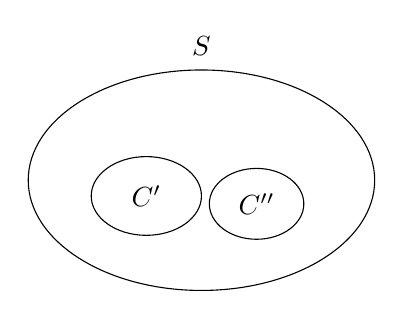
\begin{tikzpicture}
\draw (0,0) ellipse (2.2 and 1.4);
\node at (0,1.7) {$S$};
\draw (-0.7,-0.2) ellipse (0.7 and 0.5);
\draw (0.7,-0.3) ellipse (0.6 and 0.45);
\node at (-0.7,-0.2) {$C'$};
\node at (0.7,-0.3) {$C''$};
\end{tikzpicture}
\end{center}

\noindent $a\in C',\ b\in C'' \Rightarrow \hat a = C',\ \hat b = C''$. \quad $\varphi^*(\hat a,\hat b) = \varphi(a,b)$

\noindent Let $a'\in C'$ and $b'\in C''$ $\Rightarrow$ $\varphi^*(\hat a',\hat b') = \varphi(a',b')$

\bigskip
\noindent\underline{\textbf{Def:}} Let $S\neq\varnothing$, $(S,\cdot)$. An equivalence relation $R$ on $S$ is called a \textbf{congruence} on $S$ if

\noindent from $aRa'$ and $bRb' \Rightarrow abRa'b'$

\noindent (or $a\sim a'$ and $b\sim b'$) $\Rightarrow$ $(ab\sim a'b')$.

\bigskip
\noindent\underline{\textbf{Ex:}} $(\mathbb{Z},+,\cdot)$ \qquad $n \mid x-y$

\noindent $(\mathbb{Z}_n,+,\cdot)$.

\noindent $a\equiv a' \pmod n$ and $b\equiv b' \pmod n$ $\Rightarrow$ $ab\equiv a'b' \pmod n$,

\noindent $(a+b\equiv a'+b' \pmod n)$.

\[
a-a' = un,\qquad b-b'=tn
\]
\[
a+b-(a'+b') = un+tn = (u+t)n
\]
\[
ab = (a'+un)(b'+tn) = a'b' + n(\,ub'+a't+unt\,)
\]
\noindent\textit{(this last computation block is reconstructed from very small/cramped digits in the original -- please check the variables $u,t$ and the final expression.)}

\end{document}
